\documentclass[10pt, compress]{beamer}

\usetheme{glasgow}

\usepackage{booktabs}
\usepackage[scale=2]{ccicons}
\usepackage{minted}

\usepgfplotslibrary{dateplot}

\usemintedstyle{trac}

% Specify the location of images to be used
\graphicspath{{src/}}

%% Customisation
% \newcommand{\V}[1]{\v} % vectors \v{c}
% \renewcommand{\v}[1]{\mathbf{#1}} % vectors
\newcommand{\ti}[1]{\tilde{#1}} % spectral representation
\newcommand{\tnsr}[1]{\underline{\underline{#1}}}

% Symbols
\renewcommand{\O}{\omega}  % omega
\newcommand{\E}{\varepsilon}  % epsilon
\renewcommand{\u}{\mu}  % mu
\newcommand{\p}{\rho}  % rho
\newcommand{\x}{\times}  % times
\renewcommand{\inf}{\infty}  % infinity
\newcommand{\infint}{\int\limits_{-\inf}^\inf} % integral by R
\newcommand{\e}{\mathrm{e}} % Straight-up exponential
\renewcommand{\j}{{j}\mkern1mu} % Straight-up exponential
\newcommand{\iu}{\mathrm{i}\mkern1mu}

\newcommand\ddfrac[2]{\frac{\displaystyle #1}{\displaystyle #2}}





\title{High Frequency Communication Systems}
\subtitle{Lecture 1}
\date{Spring 2021}
\author{Hasan T Abbas \& Qammer H Abbasi}
% \institute{}

\begin{document}

\maketitle

\section{Preliminary Information}

\begin{frame}
  \frametitle{Course Team}
  \begin{figure}[h!]
  \subfloat[Dr Qammer H Abbasi]{
\includegraphics[width = .3\linewidth]{qammer.png}
  \label{fig:Qammer}} \hfil
  \subfloat[Dr Hasan T Abbas]{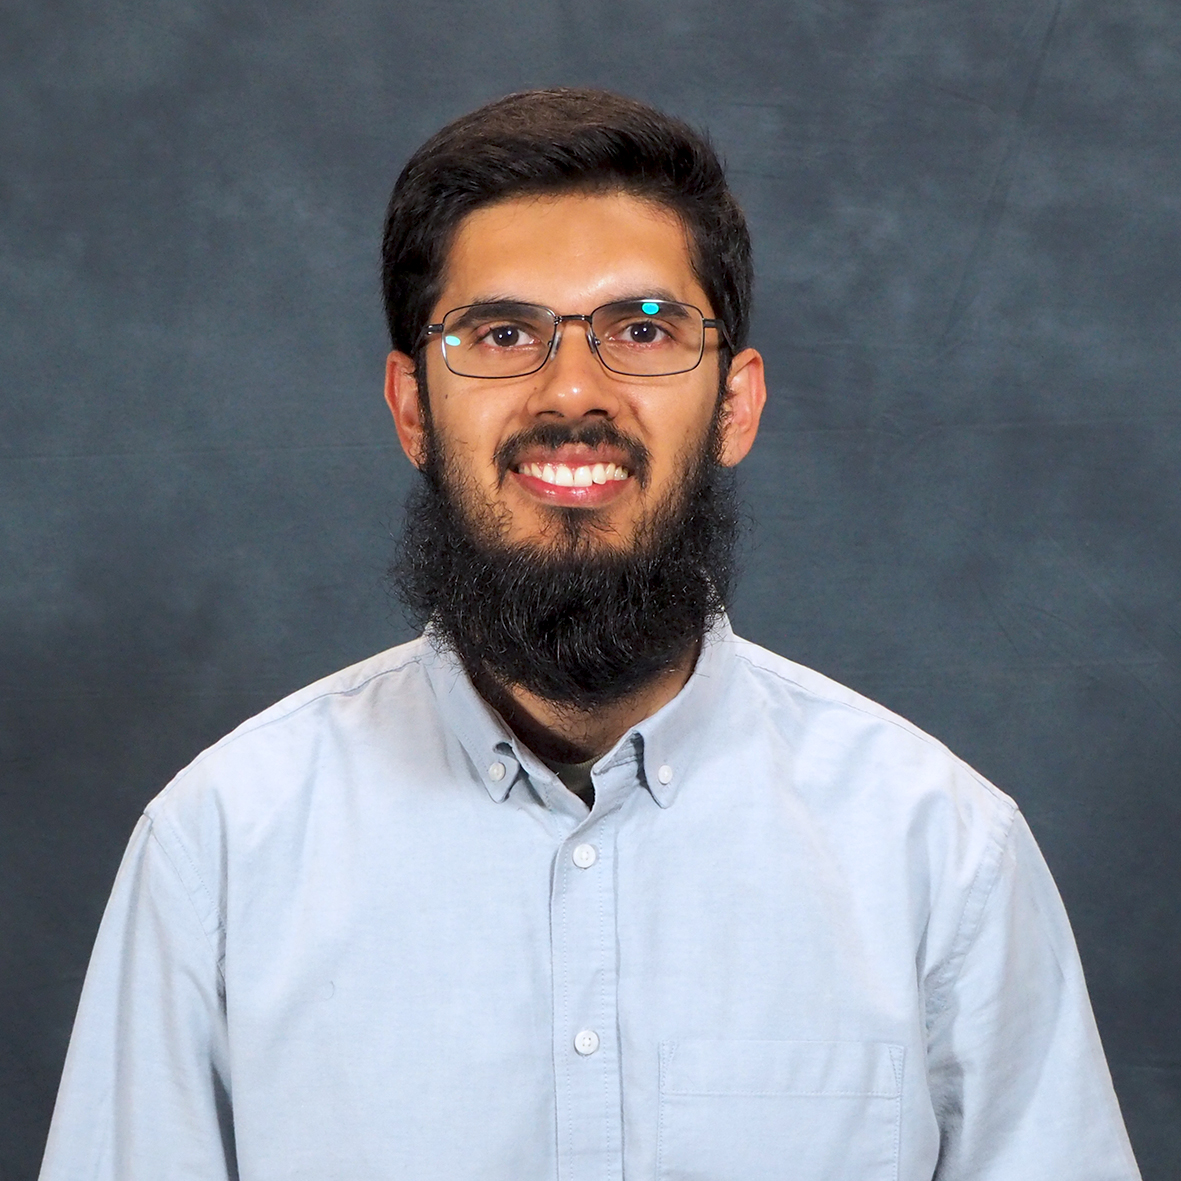
\includegraphics[width = .3\linewidth]{hasan.png}
  \label{fig:Hasan}} \hfil
  \subfloat[Mr Wenkai Jia]{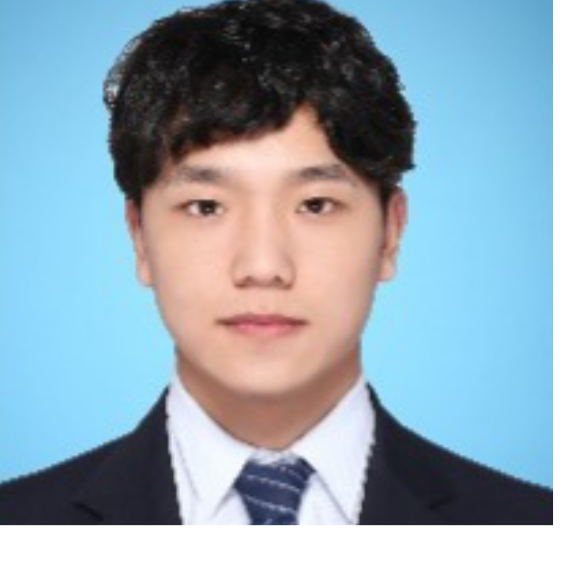
\includegraphics[width = .3\linewidth]{wenkai.png}
  \label{fig:Wenkai}} 
\end{figure}
\end{frame}
%%%%%%%%%%%%%%%%%%%%%%%%%%%%%%%%%%%%%%%%%%
%%%%%%%%%%%%%%%%%%%%%%%%%%%%%%%%%%%%%%%%%%
%%%%%%%%%%%%%%%%%%%%%%%%%%%%%%%%%%%%%%%%%%
\begin{frame}
  \frametitle{Motivation - Chang'e No. 4}
    \begin{figure}
  \centering
  
\includegraphics[width=.35\linewidth]{overthemoon.jpeg}
\end{figure}
  \begin{figure}
  \centering
  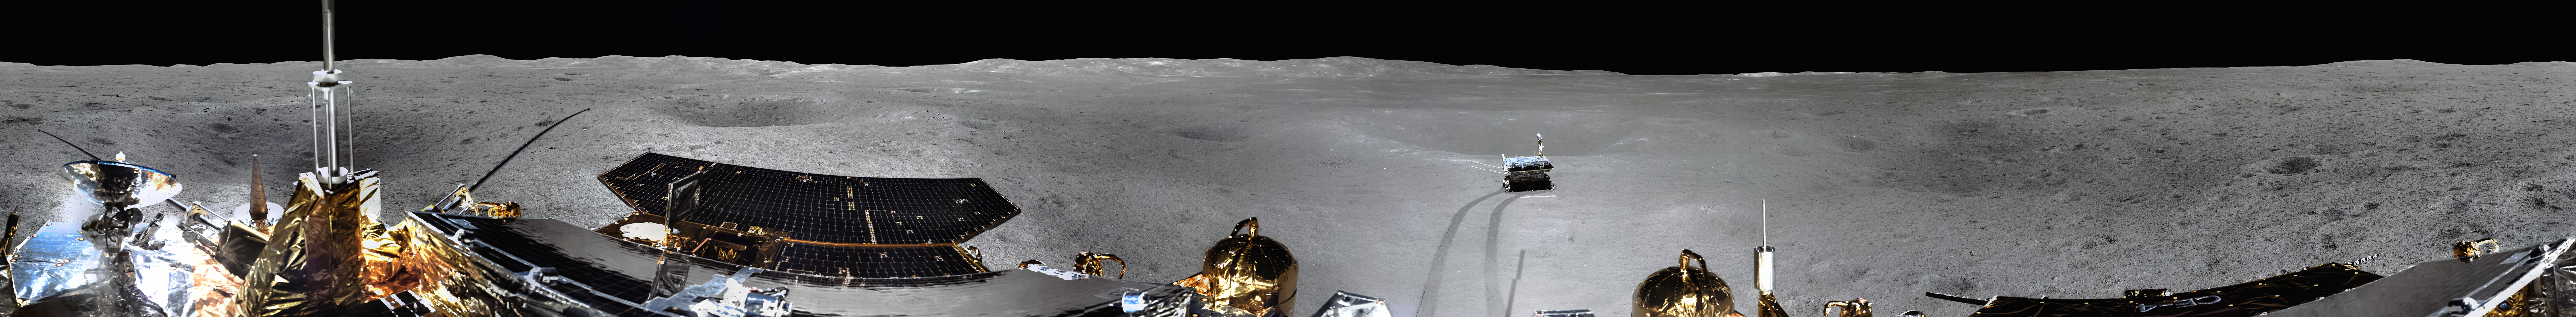
\includegraphics[width=.85\linewidth]{change.jpg}
  \caption*{Panoramic View of the Chang'e No. 4 Lander on the Moon.}
\end{figure}
\end{frame}
%%%%%%%%%%%%%%%%%%%%%%%%%%%%%%%%%%%%%%%%%%
%%%%%%%%%%%%%%%%%%%%%%%%%%%%%%%%%%%%%%%%%%
%%%%%%%%%%%%%%%%%%%%%%%%%%%%%%%%%%%%%%%%%%
\begin{frame}
  \frametitle{Course Awards}
  \begin{outline}
    \1 We will award the best students for best overall performance and best project. 
  \end{outline}
  \begin{figure}
  \subfloat[Overall Prize]{
\includegraphics[width = .45\linewidth]{gold.png}
  } \hfil
  \subfloat[Project Competition]{
\includegraphics[width = .45\linewidth]{Trophy_silver.png}}
  \end{figure}
\end{frame}
%%%%%%%%%%%%%%%%%%%%%%%%%%%%%%%%%%%%%%%%%%
%%%%%%%%%%%%%%%%%%%%%%%%%%%%%%%%%%%%%%%%%%
%%%%%%%%%%%%%%%%%%%%%%%%%%%%%%%%%%%%%%%%%%
\begin{frame}[fragile]
  \frametitle{Course Introduction}
\begin{outline}
  \1 Introduction to Millimetre wave (mmWave) and Terahertz (THz) Frequency Communication Systems
  \1 Theory of Electromagnetic (EM) wave propagation
  \1 Channel Modelling Schemes
  \1 Antenna Analysis \& Design
\end{outline}
\end{frame}
%%%%%%%%%%%%%%%%%%%%%%%%%%%%%%%%%%%%%%%%%%
%%%%%%%%%%%%%%%%%%%%%%%%%%%%%%%%%%%%%%%%%%
%%%%%%%%%%%%%%%%%%%%%%%%%%%%%%%%%%%%%%%%%%
\begin{frame}[fragile]
  \frametitle{Course Objectives}
\begin{outline}[itemize]
  \1 State of the art of electromagnetic simulation strategies for THz devices
  \1 Application of solid-state structures and novel 2D materials in mmWave and THz device technologies
  \1 Antenna design with emphasis on phased arrays used for beamforming
  \1 Wireless Propagation models of mmWave and THz communication channels
\end{outline}
\end{frame}
%%%%%%%%%%%%%%%%%%%%%%%%%%%%%%%%%%%%%%%%%%
%%%%%%%%%%%%%%%%%%%%%%%%%%%%%%%%%%%%%%%%%%
%%%%%%%%%%%%%%%%%%%%%%%%%%%%%%%%%%%%%%%%%%
\begin{frame}[fragile]
  \frametitle{Course Intended Learning Outcomes}
      At the end of the course you will be able to:
      \begin{outline}[enumerate]
        \1 Recognise the physical limitations of electromagnetic wave propagation and the need to move to higher frequencies in next generation mobile communication.
        \1 Analyse the wireless channel models to characterise a cellular communication environment.
        \1 Use electromagnetic simulation techniques to study antennas and wave propagation.
        \1 Design complex antenna systems with specific beamforming needs for mobile environments.
        \end{outline}
\end{frame}
%%%%%%%%%%%%%%%%%%%%%%%%%%%%%%%%%%%%%%%%%%
%%%%%%%%%%%%%%%%%%%%%%%%%%%%%%%%%%%%%%%%%%
%%%%%%%%%%%%%%%%%%%%%%%%%%%%%%%%%%%%%%%%%%
\begin{frame}[fragile]
  \frametitle{Course Assessments}
  \begin{table}
      \begin{tabular}{ll}
      \toprule
      Assessment & Weightage\\
      \midrule
      Homework & 30\% \\
      Exam & 20\% \\
      Lab Exercises & 20\% \\
      Lab Project \& Presentation & 20\% \\
      \bottomrule
    \end{tabular}
  \end{table}
\end{frame}
%%%%%%%%%%%%%%%%%%%%%%%%%%%%%%%%%%%%%%%%%%
%%%%%%%%%%%%%%%%%%%%%%%%%%%%%%%%%%%%%%%%%%
%%%%%%%%%%%%%%%%%%%%%%%%%%%%%%%%%%%%%%%%%%
\section{The Radio Spectrum}
\begin{frame}{Descriptions}
  \begin{figure}[t!]
  \centering
        {\includegraphics[scale=0.5]{EM.tex}
        \label{fig:EM}}
        \caption{The electromagnetic wave spectrum}
      \end{figure}
\end{frame}
%%%%%%%%%%%%%%%%%%%%%%%%%%%%%%%%%%%%%%%%%%
%%%%%%%%%%%%%%%%%%%%%%%%%%%%%%%%%%%%%%%%%%
%%%%%%%%%%%%%%%%%%%%%%%%%%%%%%%%%%%%%%%%%%
\begin{frame}
  \frametitle{Electromagnetics}
 \begin{columns}[T] % align columns
  \begin{column}{.4\textwidth}
    \begin{outline}
    \1 EM theory deals with the study of charges
    \1 Charges at rest or more importantly in motion
  \end{outline}
   \end{column}
 \begin{column}[T]{.6\textwidth}
    \begin{figure}
      \centering
          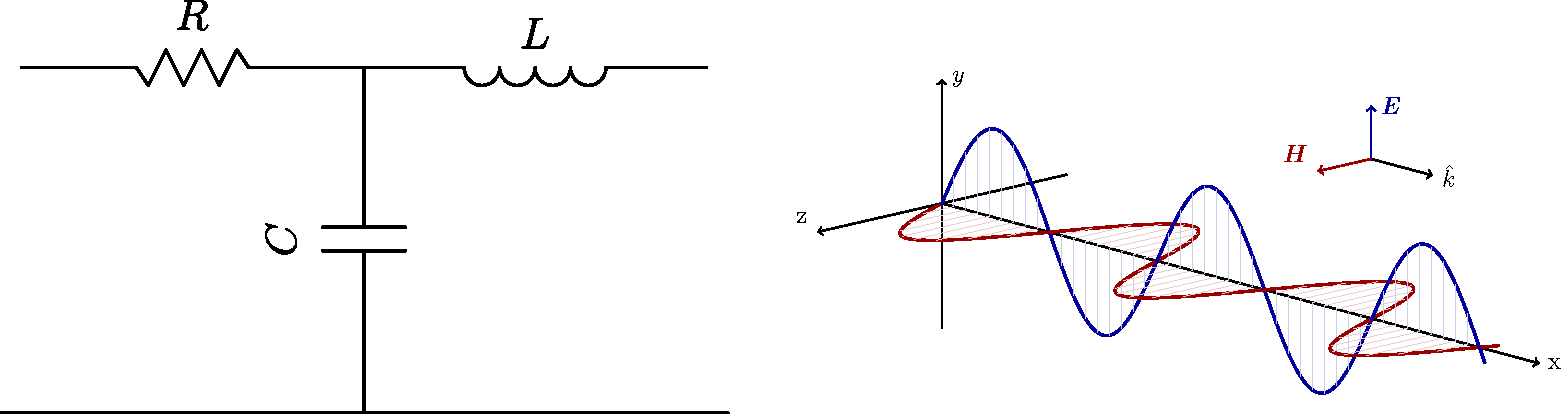
\includegraphics[width=1.0\textwidth]{em_vs_ckt.pdf}
      \caption{Circuit and Electromagnetic Theories}
    \end{figure}
      \end{column}%
\end{columns}
\begin{outline}
  \1 Circuit theory is actually a subset of EM theory
  \1 We apply \textit{lumped} circuit theory when wavelength $\lambda$ is much larger than circuit dimensions
  \2 Parasitic elements are negligible
\end{outline}
\end{frame}
%%%%%%%%%%%%%%%%%%%%%%%%%%%%%%%%%%%%%%%%%%
%%%%%%%%%%%%%%%%%%%%%%%%%%%%%%%%%%%%%%%%%%
%%%%%%%%%%%%%%%%%%%%%%%%%%%%%%%%%%%%%%%%%%
\section{The Maxwell's Equations}
\begin{frame}
    \frametitle{The Maxwell's Equations}
    \begin{outline}
      \1 Set of four linear equations
      \2 Linearity helps multiple users access one radio link (tower).
      \1 James Clerk Maxwell predicted wave propagation (1866)
      \1 Heinrich Hertz (1886) experimentally proved the results in a lab
      \1 Kick-started radio wave communications
      \1 Comprehensive in explaining EM phenomena
    \end{outline}
\end{frame}
%%%%%%%%%%%%%%%%%%%%%%%%%%%%%%%%%%%%%%%%%%
%%%%%%%%%%%%%%%%%%%%%%%%%%%%%%%%%%%%%%%%%%
%%%%%%%%%%%%%%%%%%%%%%%%%%%%%%%%%%%%%%%%%%
\begin{frame}
  \frametitle{The Maxwell's Equations - Differential Form}
  \begin{outline}
    \1 We use this form to describe the fields \textit{at any point in space and time}.
    \1 We call them field equations
    \1 Widely used to solved wave phenomena.
  \end{outline}
  \begin{align*}
\curl \va{E} &= - \pdv{\va{B}}{t} - \va{M} \tag{Faraday's Law}\\
\curl \va{H} &= \pdv{\va{D}}{t} + \va{J} \tag{Ampere's Law} \\
\div \va{E} &= \rho_e/\E_0 \tag{Gauss' Law}\\
\div \va{H} &= \rho_m/\u_0 \tag{Flux Law}
\end{align*}
\begin{outline}
  \1 The current density, $\va{J} = \va{J}_i + \va{J}_d + \va{J}_c$
  \1 In statics, $\pdv{t}$ is zero.
\end{outline}
\end{frame}
%%%%%%%%%%%%%%%%%%%%%%%%%%%%%%%%%%%%%%%%%%
%%%%%%%%%%%%%%%%%%%%%%%%%%%%%%%%%%%%%%%%%%
%%%%%%%%%%%%%%%%%%%%%%%%%%%%%%%%%%%%%%%%%%
\begin{frame}
  \frametitle{The Maxwell's Equations - Integral Form}
  \begin{outline}
    \1 We use this form to describe the fields over \textit{an extended region of space}.
    \1 Not widely used.
  \end{outline}
  \begin{align*}
  \oint_{C} \va{E} \cdot \dd{\va{l}}  &= -\pdv{t} \iint_{S} \va{B} \cdot \dd{\va{S}} \tag{Faraday's Law} \\
  \oint_{C} \va{H} \cdot \dd{\va{l}}  &= \iint_{S} \va{J} \cdot \dd{\va{S}}  + \pdv{t} \iint_{S} \va{D} \cdot \dd{\va{S}} \tag{Ampere's Law}\\
  \oiint_{S} \va{D} \cdot \dd{\va{S}} &= \iiint_{V} \p_e \dd{V}
  = \phi_e \tag{Gauss' Law} \\
  \oiint_{S} \va{B} \cdot \dd{\va{S}}  &= \iiint_{V} \p_m \dd{V}
  = \phi_m \tag{Flux Law}
\end{align*}
\end{frame}
%%%%%%%%%%%%%%%%%%%%%%%%%%%%%%%%%%%%%%%%%%
%%%%%%%%%%%%%%%%%%%%%%%%%%%%%%%%%%%%%%%%%%
%%%%%%%%%%%%%%%%%%%%%%%%%%%%%%%%%%%%%%%%%%
\begin{frame}
  \frametitle{Constitutive Relationships - Simple Materials}
    How the flux densities (electric $\va{D}$, magnetic $\va{B}$) and field intensities (electric $\va{E}$, magnetic $\va{H}$) are related.

  For simple (isotropic) materials, we have a simple linear relationship:
  \begin{align*}
    \va{D} &= \E \va{E} \; [\si{\coulomb \per \m \squared}] \tag{Dielectric Material} \\
    \va{B} &= \u \va{H} \; [\si{\weber \per \m \squared}] \tag{Magnetic Material} \\
    \va{J} &= \sigma \va{E} \; [\si{\ampere \per \m \squared}]
  \end{align*}
  \begin{outline}
    \1 $\E$ and $\u$ are the permittivity and permeability of a given material respectively. For simple (isotropic and homogeneous) materials, these are real numbers.
    \1 At higher frequencies, we need to consider the material polarizability.
  \end{outline}

\end{frame}
%%%%%%%%%%%%%%%%%%%%%%%%%%%%%%%%%%%%%%%%%%
%%%%%%%%%%%%%%%%%%%%%%%%%%%%%%%%%%%%%%%%%%
%%%%%%%%%%%%%%%%%%%%%%%%%%%%%%%%%%%%%%%%%%
\begin{frame}
  \frametitle{Further Material Properties}

\begin{outline}
  \1 We can extract many material properties from $\E$ and $\u$.
\end{outline}
The speed of light:
  \begin{align*}
    c &= \sqrt{\frac{1}{\u \E}}
  \end{align*}

The characteristic impedance:
\begin{align*}
    \eta &= \sqrt{\frac{\u}{\E}}
  \end{align*}

The refractive index:
\begin{align*}
    n &= \sqrt{{\u}{\E}}
  \end{align*}

  \begin{outline}
    \1 Most materials are considered non-magnetic ($\u_r = 1$).
    \1 Further properties at nanoscale EM
  \end{outline}
\end{frame}
%%%%%%%%%%%%%%%%%%%%%%%%%%%%%%%%%%%%%%%%%%
%%%%%%%%%%%%%%%%%%%%%%%%%%%%%%%%%%%%%%%%%%
%%%%%%%%%%%%%%%%%%%%%%%%%%%%%%%%%%%%%%%%%%
\begin{frame}
  \frametitle{Some Complex Materials}

In real life, there are many types of media. Generally,
\begin{align*}
  \va{D}(\va{r}, t) &= \E(\va{r}) \va{E}(\va{r}, t)  [\si{\coulomb \per \m \squared}]
\end{align*}

Anisotropic materials:
\begin{align*}
\begin{bmatrix}
D_{x} \\
D_{y} \\
D_{z}
\end{bmatrix}
=
\begin{bmatrix}
\E_{x x} & \E_{x y} & \E_{x z} \\
\E_{y x} & \E_{y y} & \E_{y z} \\
\E_{z x} & \E_{z y} & \E_{z z}
\end{bmatrix}
\begin{bmatrix}
E_{x} \\
E_{y} \\
E_{z}
\end{bmatrix}
\end{align*}

The permittivity $\E$ is a tensor (or matrix) as properties depend on the direction.

For media with loss, $\E$ is a complex number.
\end{frame}
%%%%%%%%%%%%%%%%%%%%%%%%%%%%%%%%%%%%%%%%%%
%%%%%%%%%%%%%%%%%%%%%%%%%%%%%%%%%%%%%%%%%%
%%%%%%%%%%%%%%%%%%%%%%%%%%%%%%%%%%%%%%%%%%
\begin{frame}
\frametitle{Dispersive Media}
\begin{columns}[T] % align columns
  \begin{column}{.4\textwidth}
\begin{outline}
  \1 For dispersive media, \textcolor{red}{$\E = f(\O)$}.
  \2 Unsuitable for communications
  \3 Material Dispersion causes pulse spreading
  \1 We compute the dispersion relation for devices such as waveguides.
  \1 However, naturally all materials are dispersive to some extent.
\end{outline}
   \end{column}
 \begin{column}[T]{.6\textwidth}
        \begin{figure}
      \centering
          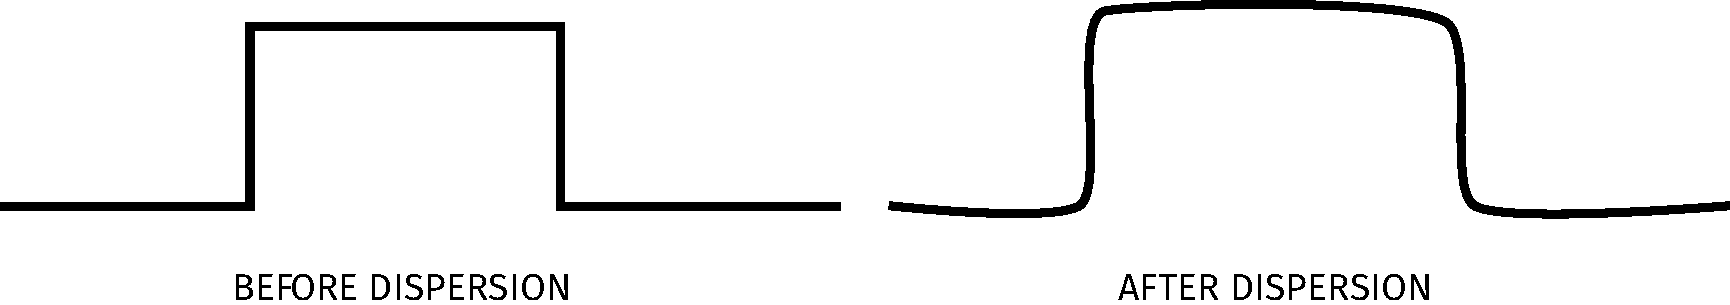
\includegraphics[width=1.0\textwidth]{DISPERSION.pdf}
      \caption{Frequency Dispersion}
    \end{figure}
  \end{column}%
\end{columns}
\end{frame}
%%%%%%%%%%%%%%%%%%%%%%%%%%%%%%%%%%%%%%%%%%
%%%%%%%%%%%%%%%%%%%%%%%%%%%%%%%%%%%%%%%%%%
%%%%%%%%%%%%%%%%%%%%%%%%%%%%%%%%%%%%%%%%%%
\begin{frame}
\frametitle{Circuit Theory and Field Equations}
\begin{outline}
  \1 Common circuit laws (Ohm's, KCL, and KVL) can be derived from the Maxwell's equations
  \1 All circuit relations can be extracted
\end{outline}
\begin{align*}
  \va{J}_c &=\sigma \va{E} &\quad \Leftrightarrow \quad i &=\frac{1}{R} v_{R} = G v_{R} \tag{Ohm's Law} \\
\va{B} & = \u \va{H} &\quad \Leftrightarrow \quad \phi_{m} &= L i_{L} \\
\va{M} &= \u \pdv{\va{H}}{t} &\quad \Leftrightarrow \quad v_{L}&= L \pdv{i_L}{t} \\
\va{D} &= \E \va{E} &\quad \Leftrightarrow \quad  Q &= C v \\
\va{J}_d &= \E \pdv{\va{E}}{t} &\quad \Leftrightarrow \quad i_{C} &= C \pdv{v}{t}
\end{align*}
\end{frame}
%%%%%%%%%%%%%%%%%%%%%%%%%%%%%%%%%%%%%%%%%%
%%%%%%%%%%%%%%%%%%%%%%%%%%%%%%%%%%%%%%%%%%
%%%%%%%%%%%%%%%%%%%%%%%%%%%%%%%%%%%%%%%%%%
\begin{frame}
  \frametitle{Deriving Circuit Relations - KVL}
      \begin{align*}
      \oint_{C} \va{E} \cdot \dd{\va{l}} =- \pdv{t} \iint_{S} \va{B} \cdot \dd{\va{S}} =-\pdv{\phi_m}{t} \Leftrightarrow \sum v = -\pdv{\phi_m}{t} = -L_{s} \pdv{i}{t}
    \end{align*}
    \begin{align*}
      -V + V_R + V_L + V_C  =& -L_{s} \pdv{i}{t}
    \end{align*}
    \begin{figure}
            \centering
          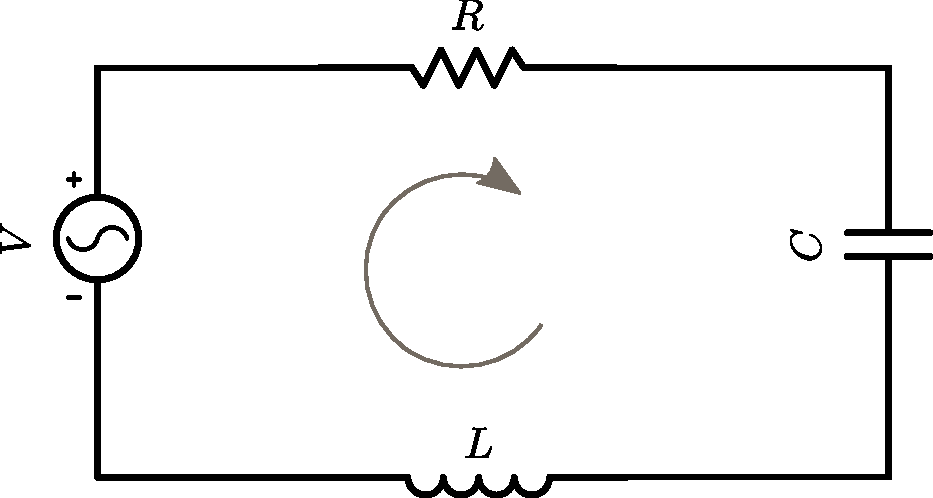
\includegraphics[width=.4\textwidth]{circuit.pdf}
      \caption{A Simple Circuit}
    \end{figure}
    \begin{outline}
      \1 $L_s = 0$ when circuit dimensions are much smaller than the wavelength ($\implies \sum v = 0$).
    \end{outline}
\end{frame}
%%%%%%%%%%%%%%%%%%%%%%%%%%%%%%%%%%%%%%%%%%
%%%%%%%%%%%%%%%%%%%%%%%%%%%%%%%%%%%%%%%%%%
%%%%%%%%%%%%%%%%%%%%%%%%%%%%%%%%%%%%%%%%%%
\begin{frame}
  \frametitle{Circuit and Field Concept Correspondence}
\begin{table}
      \begin{tabular}{ll}
      \toprule
      Circuit & Field\\
      \midrule
      Voltage $V$ & Electric Field Intensity $\va{E}$ \\
      Current $I$ & Magnetic Field Intensity $\va{H}$  \\
      Power $V \times I^{*}$ & Poynting Vector Power Flow $\va{E} \times \va{H}^*$ \\
      Lab Project \& Presentation & 20\% \\
      \bottomrule
    \end{tabular}
  \end{table}
\end{frame}
%%%%%%%%%%%%%%%%%%%%%%%%%%%%%%%%%%%%%%%%%%
%%%%%%%%%%%%%%%%%%%%%%%%%%%%%%%%%%%%%%%%%%
%%%%%%%%%%%%%%%%%%%%%%%%%%%%%%%%%%%%%%%%%%
\begin{frame}
  \frametitle{Boundary Conditions}
  You may have noticed loss of cell-phone reception when inside an elevator or driving through a tunnel.

  EM wave propagation is governed by \textcolor{red}{boundary conditions}.
  \begin{outline}
    \1 We are interested in determining the fields in a given region in space
    \2 Use the integral forms to derive the boundary conditions
    \1 Boundaries represent discontinuities in field values
    \2 The derivatives become undefined
    \1 We break the fields into \textit{tangential} and \textit{normal} components
  \end{outline}
\end{frame}
%%%%%%%%%%%%%%%%%%%%%%%%%%%%%%%%%%%%%%%%%%
%%%%%%%%%%%%%%%%%%%%%%%%%%%%%%%%%%%%%%%%%%
%%%%%%%%%%%%%%%%%%%%%%%%%%%%%%%%%%%%%%%%%%
\begin{frame}
  \frametitle{Boundary Conditions}
  \begin{figure}
    \centering
          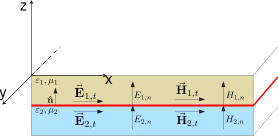
\includegraphics[width=.9\textwidth]{BC.pdf}
      \caption{Boundary Conditions at an Interface}
  \end{figure}
\end{frame}
%%%%%%%%%%%%%%%%%%%%%%%%%%%%%%%%%%%%%%%%%%
%%%%%%%%%%%%%%%%%%%%%%%%%%%%%%%%%%%%%%%%%%
%%%%%%%%%%%%%%%%%%%%%%%%%%%%%%%%%%%%%%%%%%
\begin{frame}
  \frametitle{Boundary Conditions}
  \begin{outline}
    \1 The tangential components of the fields remain continuous along the boundary
    \1 The normal components are discontinuous
  \end{outline}
  \begin{align*}
    \vu{n} \cross (\va{E}_1 - \va{E}_2) &= \va{M}_s \\
    \vu{n} \cdot (\va{D}_2 - \va{D}_1) &= \p_{e,s} \\
  \end{align*}
  Similarly,
  \begin{align*}
     \vu{n} \cross (\va{H}_1 - \va{H}_2) &= -\va{J}_s \\
    \vu{n} \cdot (\va{B}_2 - \va{B}_1) &= \p_{m,s} \\
  \end{align*}
\end{frame}
%%%%%%%%%%%%%%%%%%%%%%%%%%%%%%%%%%%%%%%%%%
%%%%%%%%%%%%%%%%%%%%%%%%%%%%%%%%%%%%%%%%%%
%%%%%%%%%%%%%%%%%%%%%%%%%%%%%%%%%%%%%%%%%%
\begin{frame}
  \frametitle{Boundary Conditions - Special Cases}
  \begin{outline}
    \1 For finite conductivity media ($\sigma_1, \sigma_2 \neq \inf$)
      \2 $\va{J}_s, \va{M}_s = 0$, $\p_{e,s}, \p_{m,s} = 0$
  \end{outline}
  \begin{align*}
    \vu{n} \cross (\va{E}_1 - \va{E}_2) &= 0 \\
    \vu{n} \cross (\va{H}_2 - \va{H}_1) &= 0 \\
    \vu{n} \cdot (\va{D}_2 - \va{D}_1) &= 0 \\
    \vu{n} \cdot (\va{B}_2 - \va{B}_1) &= 0 \\
  \end{align*}
\end{frame}
%%%%%%%%%%%%%%%%%%%%%%%%%%%%%%%%%%%%%%%%%%
%%%%%%%%%%%%%%%%%%%%%%%%%%%%%%%%%%%%%%%%%%
%%%%%%%%%%%%%%%%%%%%%%%%%%%%%%%%%%%%%%%%%%
\begin{frame}
  \frametitle{Boundary Conditions - Special Cases}
  \begin{outline}
    \1 For one PEC medium  ($\sigma_1 = \inf$)
      \2 $\va{E_1} = \va{H_1} = 0$, All magnetic sources are zero
  \end{outline}
  \begin{align*}
    \vu{n} \cross \va{E}_2 &= 0 \\
    \vu{n} \cdot \va{H}_2 &= \va{J}_s \\
    \vu{n} \cdot \va{D} &= \p_{e,s} \\
    \vu{n} \cdot \va{B}_2 &= 0 \\
  \end{align*}
\end{frame}
%%%%%%%%%%%%%%%%%%%%%%%%%%%%%%%%%%%%%%%%%%
%%%%%%%%%%%%%%%%%%%%%%%%%%%%%%%%%%%%%%%%%%
%%%%%%%%%%%%%%%%%%%%%%%%%%%%%%%%%%%%%%%%%%
\begin{frame}
  \frametitle{Time Harmonic Fields}
  \begin{outline}
    \1 In majority of cases, the time-variance of the fields is sinusoidal (time-harmonic).
    \1 These time variations represented by $\exp(\j \omega t)$
    \1 We replace $\pdv*{}{t}$ by $\j \omega$.
  \end{outline}
  \begin{align*}
    \curl{\va{E}} &= -\j \omega \va{B} \\
     \curl{\va{H}} &= \j \omega \E \va{E} + \va{J} \\
     \div{\va{E}} &= \p/\E \\
     \div{\va{H}} &= 0
  \end{align*}
\end{frame}
%%%%%%%%%%%%%%%%%%%%%%%%%%%%%%%%%%%%%%%%%%
%%%%%%%%%%%%%%%%%%%%%%%%%%%%%%%%%%%%%%%%%%
%%%%%%%%%%%%%%%%%%%%%%%%%%%%%%%%%%%%%%%%%%
\begin{frame}
  \frametitle{Next Lecture}
  \begin{outline}
    \1 Wave Equations
    \1 Dielectric Properties and Materials
    \1 Nano-scale Electromagnetics
  \end{outline}
\end{frame}
\end{document}
